\subsection{Run by Run Jet QA}

The QA of reconstructed jets in this study is assessed by analyzing the average number of jets per event and the average jet energy per event. 
The event selections outlined in Section \ref{sec:selection} are implemented before analyzing these QA plots.

Figures~\ref{fig:avgNjet} and \ref{fig:avgEjet} show the distributions of the average number of jets per event and the average energy of jets per event, respectively. 
These distributions are evaluated for each run using the following additional criteria:
\begin{itemize}
    \item Jet transverse momentum: \( p_T > 5~\text{GeV} \)
    \item Trigger selection: Events must be associated with jet 10 trigger - scaled trigger bit 22
    \item Both jets must be central, with \( |\eta| < 0.7 \)
    \item Leading jet uncalibrated transverse momentum: \( p_T^{\text{lead}} \geq 15~\text{GeV} \)
    \item Subleading jet uncalibrated transverse momentum: \( p_T^{\text{sublead}} \geq 0.3~p_T^{\text{lead}} \)
    \item Leading and subleading jet with \( |\Delta\phi| \geq 3\pi/4 \)
\end{itemize}

\begin{figure}
    \centering
    \begin{subfigure}[t]{0.48\textwidth}
        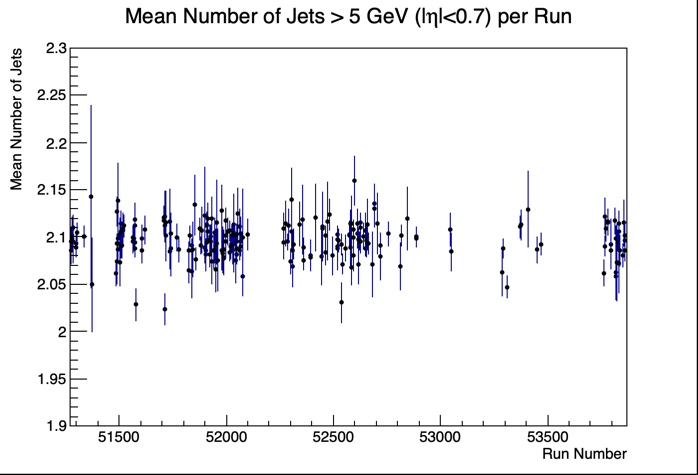
\includegraphics[width=\linewidth, trim=10 10 10 0, clip]{Figures/QA_Study/avg_njet_case7.png}
        \caption{Average number of jets per event after all selection criteria.}\label{fig:avgNjet}
    \end{subfigure}
    \hfill
    \begin{subfigure}[t]{0.48\textwidth}
        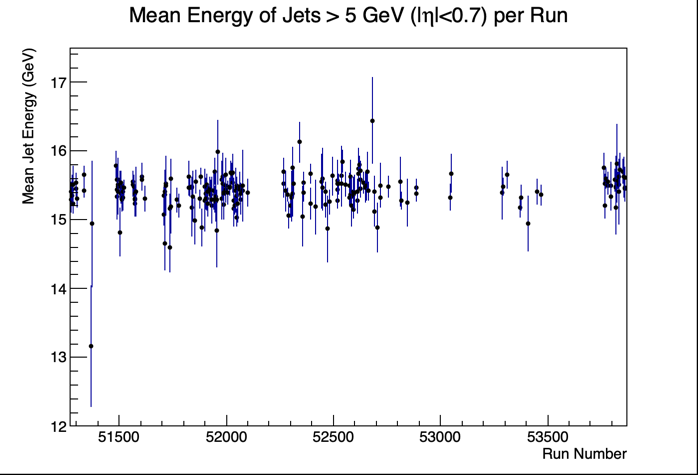
\includegraphics[width=\linewidth, trim=10 10 10 0, clip]{Figures/QA_Study/avg_ejet_case7.png}
        \caption{Average energy of jets per event after all selection criteria.}\label{fig:avgEjet}
    \end{subfigure}
    \caption{Jet QA observables: (a) average number of jets per event and (b) average jet energy, after all selection cuts.}
    \label{fig:qa_jet_summary}
\end{figure}
The results indicate that, on average, two jets are reconstructed per event, and the average jet energy is approximately 15.5~GeV.

\subsection{Run by Run Calorimeter Tower and Cluster QA}

To evaluate the stability and quality of the calorimeter response during data-taking, a performance study was conducted for jet events triggered with scaled triggers which correspond to the Jet 8, Jet 10 and Jet 12 trigger bits with (trigger bits 16, 17, 18, 33, 34, 35) and without (trigger bits 21, 22, 23) the online MBD coincidence requirement.  
In each of these jet events, the same selection criteria as outlined in Section \ref{sec:selection} and applied in the jet QA study are applied here for the calorimeter tower studies.
The analysis focused mainly on the reconstructed level average total transverse energy per event in each of the three jet event regions: towards, transverse, and away.
This study was preformed using calorimeter towers, EMCal clusters and topoclusters to understand the stability of these reconstruction methods to noise changes over the course of Run 2024 p+p running.

\subsubsection{Average Total Transverse Energy from Topoclusters}
The average transverse energy per event based on topoclusters was evaluated as a function of run number for events selected with selection criteria outlined above. 
In the towards region, the average transverse energy is approximately 18~GeV, while in the transverse region it is around 1.4~GeV. In the away region, the average transverse energy is about 14~GeV. 
These values are stable across the run range, indicating good performance of the topocluster-based reconstruction under the applied selection conditions.
\begin{figure}
    \centering
    \begin{subfigure}[t]{0.32\linewidth}
        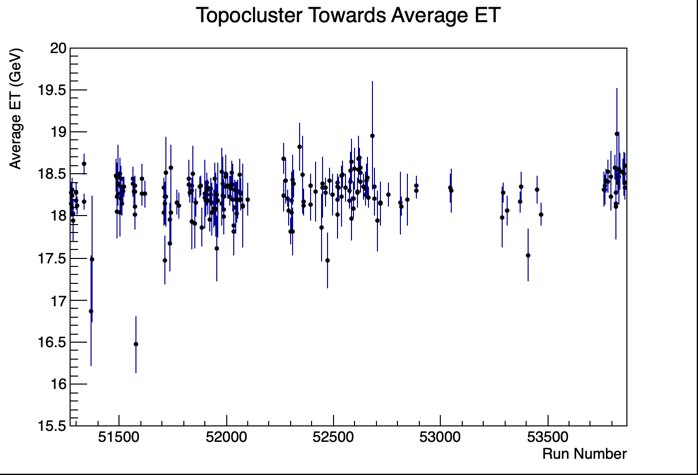
\includegraphics[width=\linewidth, trim=10 10 10 0, clip]{Figures/QA_Study/avg_et_topo_towards_case4.png}
        \caption{Towards region}
        \label{fig:et_topo_towards_case4}
    \end{subfigure}
    \hfill
    \begin{subfigure}[t]{0.32\linewidth}
        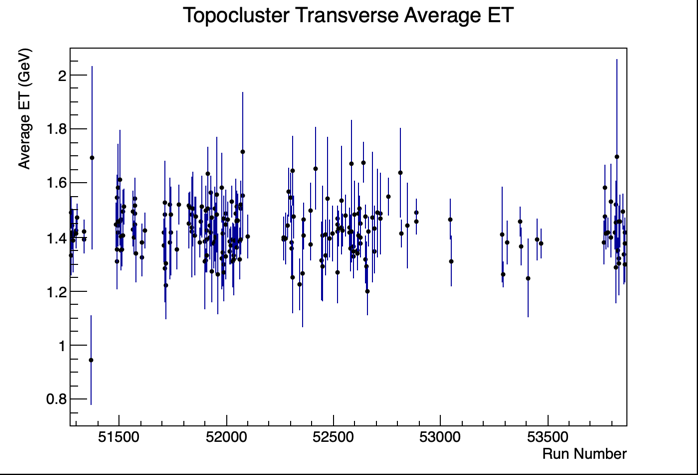
\includegraphics[width=\linewidth, trim=10 10 10 0, clip]{Figures/QA_Study/avg_et_topo_transverse_case4.png}
        \caption{Transverse region}
        \label{fig:et_topo_transverse_case4}
    \end{subfigure}
    \hfill
    \begin{subfigure}[t]{0.32\linewidth}
        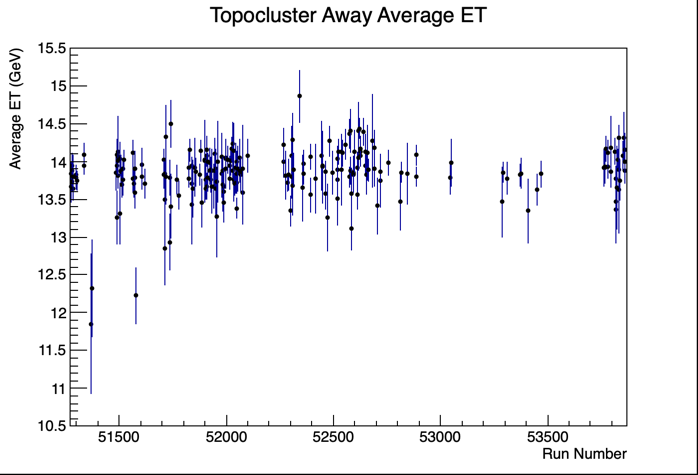
\includegraphics[width=\linewidth, trim=10 10 10 0, clip]{Figures/QA_Study/avg_et_topo_away_case4.png}
        \caption{Away region}
        \label{fig:et_topo_away_case4}
    \end{subfigure}
    \caption{Average transverse energy from topoclusters versus run number for (a) towards, (b) transverse, and (c) away regions.}
    \label{fig:avg_et_topo_case4}
\end{figure}

\subsubsection{Average Total Transverse Energy from EMCal Clusters}

To further evaluate the energy deposition patterns using a different reconstruction approach, the average transverse energy per event was studied using EMCal clusters~\cite{Seidlitz1} rather than towers. 
Here there are two obvious trends: the average transverse energy all three regions is much higher than the same observable reconstructed using just EMCal towers (see Fig~\ref{fig:calo_tower_et_regions}) and the the average transverse energy all three regions grows considerably over the course of the Run. 
The EMCal clusters are highly noise dominated since they do not have a seeding requirement in the same way as the topoclusters and the tower threshold for the EMCal cluster reconstruction is set right in the middle of the noise spectrum at a value of 70 MeV. Therefore, the average total transverse region \ET{} extracted from EMCal clusters is 5 times that extracted from EMCal towers (Fig~\ref{fig:calo_tower_et_regions}) and changes 35\% over the course of the Run.
The nominal EMCal cluster threshold set in the middle of the noise spectrum combined with the EMCal clustering algorithm not having a higher seed threshold for noise reduction (like the topoclusters) makes the average transverse energy from EMCal clusters not a good noise-insensitive proxy for the average transverse energy. 

\begin{figure}
    \centering
    \begin{subfigure}[t]{0.32\linewidth}
        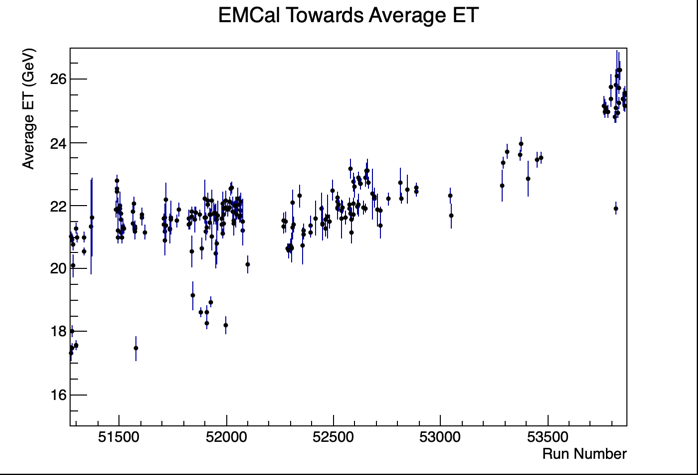
\includegraphics[width=\linewidth, trim=10 10 10 0, clip]{Figures/QA_Study/avg_et_cluster_towards_case4.png}
        \caption{Towards region}
        \label{fig:et_cluster_towards_case4}
    \end{subfigure}
    \hfill
    \begin{subfigure}[t]{0.32\linewidth}
        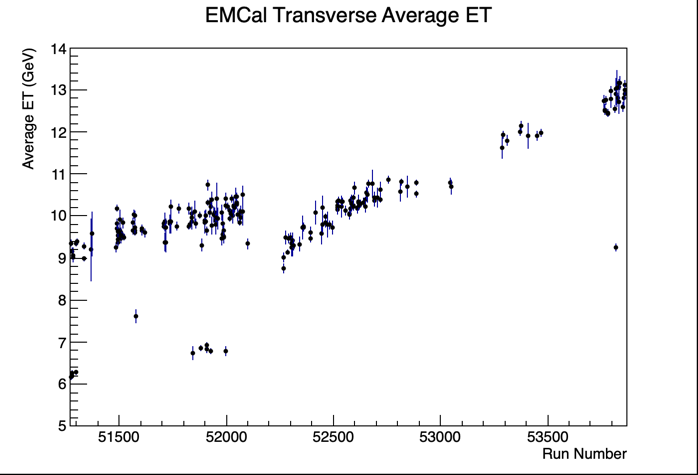
\includegraphics[width=\linewidth, trim=10 10 10 0, clip]{Figures/QA_Study/avg_et_cluster_transverse_case4.png}
        \caption{Transverse region}
        \label{fig:et_cluster_transverse_case4}
    \end{subfigure}
    \hfill
    \begin{subfigure}[t]{0.32\linewidth}
        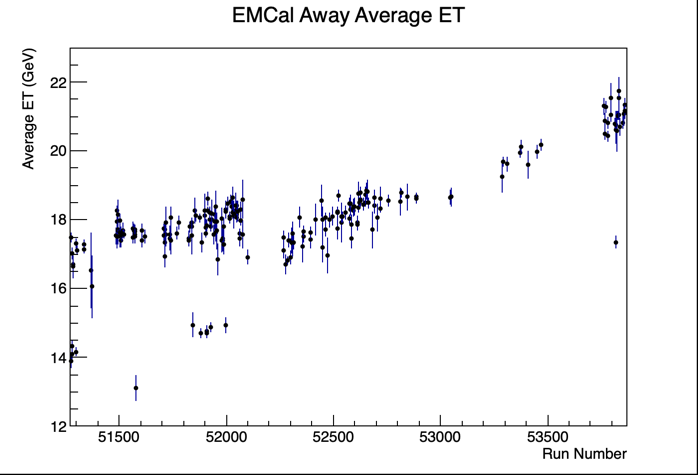
\includegraphics[width=\linewidth, trim=10 10 10 0, clip]{Figures/QA_Study/avg_et_cluster_away_case4.png}
        \caption{Away region}
        \label{fig:et_cluster_away_case4}
    \end{subfigure}
    \caption{Average transverse energy from EMCal clusters versus run number in the (a) towards, (b) transverse, and (c) away regions.}
    \label{fig:avg_et_cluster_case4}
\end{figure}

\subsubsection{Average Total Transverse Energy from Calorimeter Towers}

Finally, the average total transverse energy from calorimeter towers was evaluated calorimeter layer by layer in the three jet event regions.
The average transverse energy from each layer is shown in Figure~\ref{fig:emcal_et_regions} for the EMCal, Figure~\ref{fig:ihcal_et_regions} for the IHCal, and Figure~\ref{fig:ohcal_et_regions} for the OHCal.
The EMCal transverse region average energy is around 2~GeV which is higher than the average transverse energy from topoclusters but much lower than the average transverse energy from EMCal clusters.

There is also a small run dependence ($\sim15\%$) in the EMCal transverse region average energy which is likely due to the noise variations in the EMCal over the course of the run and the processing of noise waveforms using the template fit method.
Therefore, while EMCal towers are less sensitive to noise changes over the course of the run than EMCal clusters, they are still not as good of a noise-insensitive proxy for the average transverse energy as the topoclusters with optimized noise thresholds.
The IHCal and OHCal transverse region average energies are around 0.2~GeV and 0.5~GeV respectively which is much lower than the average transverse energy from EMCal clusters.
Additionally, the IHCal and OHCal have lower overall noise and saw less noise variation over the course of the Run then the EMCal.
Therefore, the IHCal and OHCal transverse region average energies are more stable over the course of the run than the EMCal transverse region average energy.

\begin{figure}
    \centering
    \begin{subfigure}[t]{\textwidth}
        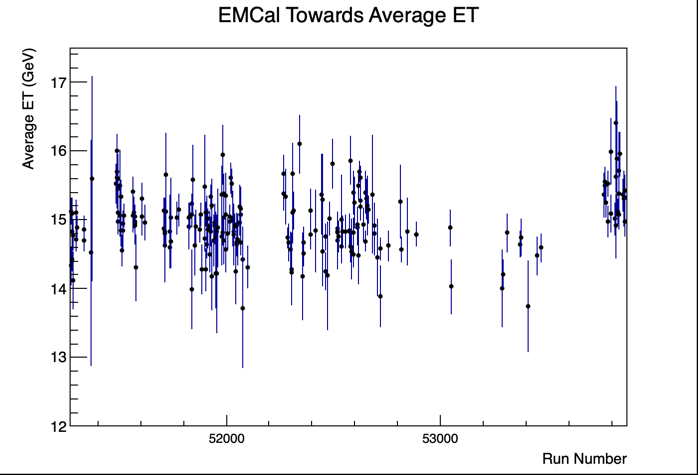
\includegraphics[width=0.32\linewidth]{Figures/QA_Study/avg_et_emcal_towards_case5.png}
        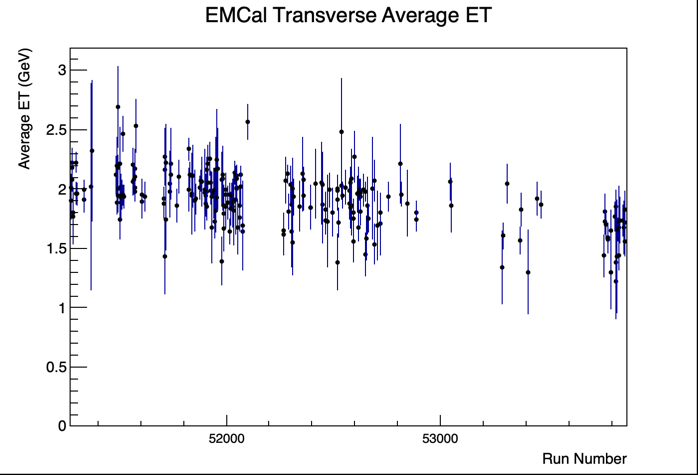
\includegraphics[width=0.32\linewidth]{Figures/QA_Study/avg_et_emcal_transverse_case5.png}
        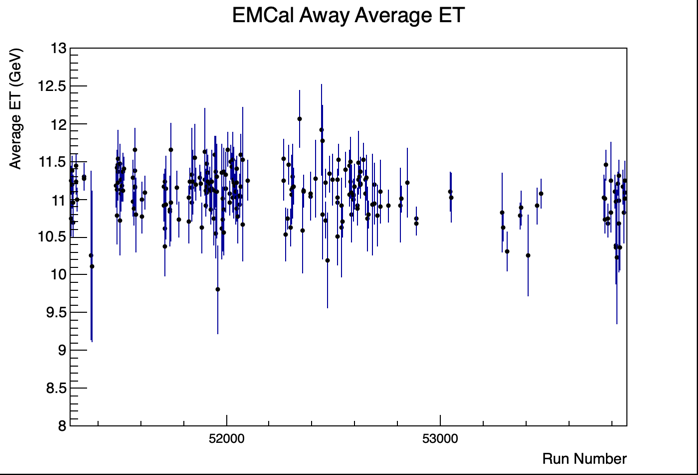
\includegraphics[width=0.32\linewidth]{Figures/QA_Study/avg_et_emcal_away_case5.png}
        \caption{EMCal: Towards, Transverse, and Away regions}
        \label{fig:emcal_et_regions}
    \end{subfigure}
    \hfill
    \begin{subfigure}[t]{\textwidth}
        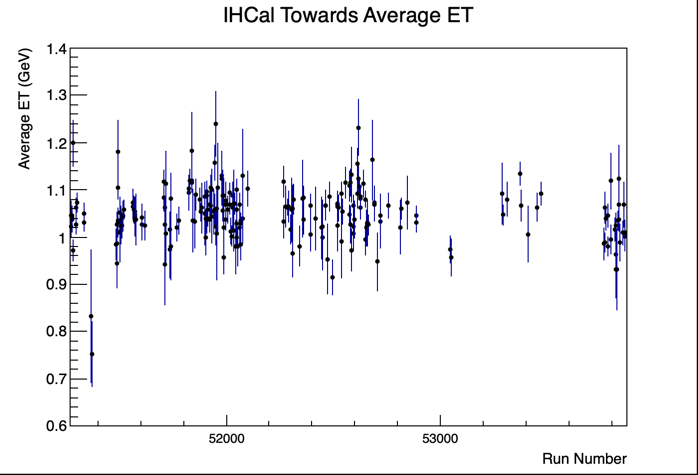
\includegraphics[width=0.32\linewidth]{Figures/QA_Study/avg_et_ihcal_towards_case5.png}
        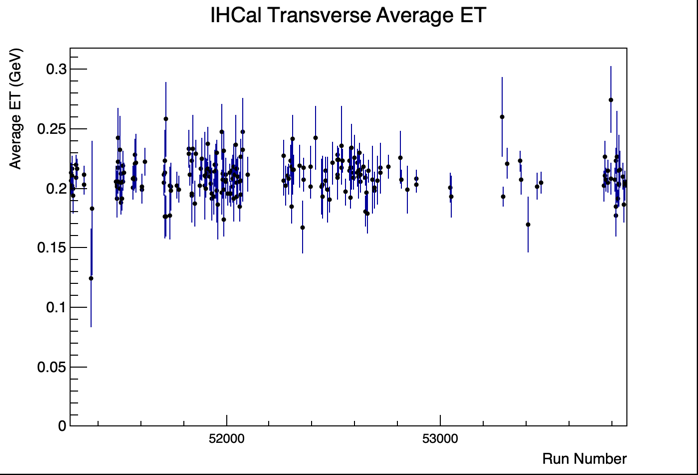
\includegraphics[width=0.32\linewidth]{Figures/QA_Study/avg_et_ihcal_transverse_case5.png}
        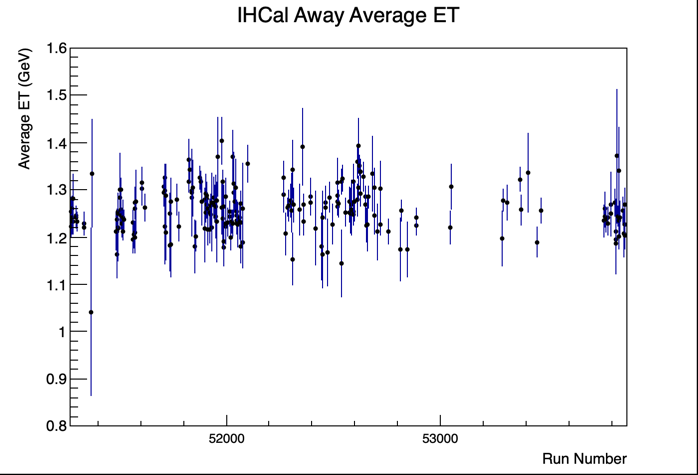
\includegraphics[width=0.32\linewidth]{Figures/QA_Study/avg_et_ihcal_away_case5.png}
        \caption{IHCal: Towards, Transverse, and Away regions}
        \label{fig:ihcal_et_regions}
    \end{subfigure}
    \hfill
    \begin{subfigure}[t]{\textwidth}
        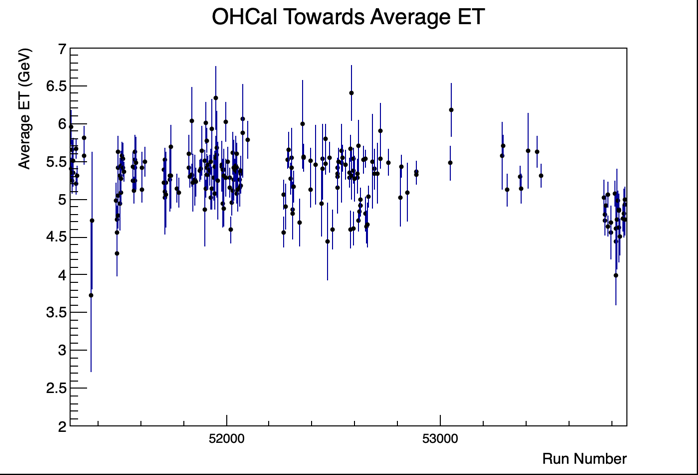
\includegraphics[width=0.32\linewidth]{Figures/QA_Study/avg_et_ohcal_towards_case5.png}
        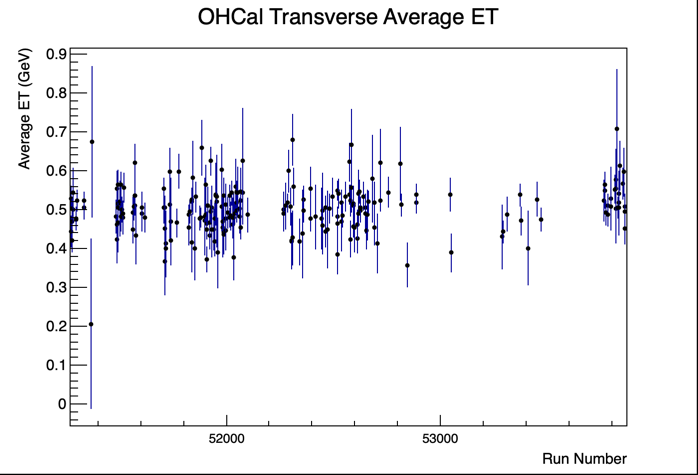
\includegraphics[width=0.32\linewidth]{Figures/QA_Study/avg_et_ohcal_transverse_case5.png}
        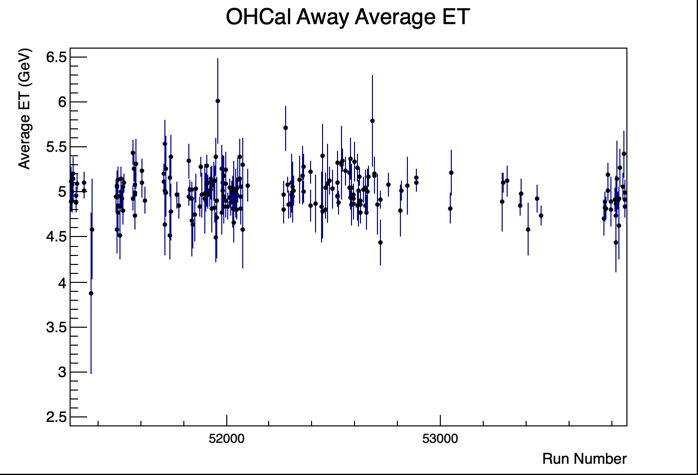
\includegraphics[width=0.32\linewidth]{Figures/QA_Study/avg_et_ohcal_away_case5.png}
        \caption{OHCal: Towards, Transverse, and Away regions}
        \label{fig:ohcal_et_regions}
    \end{subfigure}
    \caption{Average transverse energy in EMCal (top), IHCal (middle) and OHCal (bottom) in the towards (left), transverse (middle), and away (right) regions.}
    \label{fig:calo_tower_et_regions}
\end{figure}
